% Preamble
\documentclass{article}

% Packages
\usepackage[legalpaper, portrati, margin=0.9in]{geometry}
\usepackage{amsmath}
\usepackage{bm}
\usepackage{amssymb}
\usepackage{gensymb}
\usepackage{mathtools}
\usepackage{xcolor}
\usepackage{caption}
\usepackage{subcaption}
\usepackage{pgfplots}
\pgfplotsset{compat=1.17}
\usepackage{tikz}
\usepackage{tkz-euclide}


% Macros
\DeclareMathOperator{\arcsec}{arcsec}
\DeclareMathOperator{\arccot}{arccot}
\DeclareMathOperator{\arccsc}{arccsc}


% File info
\title{Calculus Notes}
\author{Eric Xia}
\date{Last Updated 10 June 2020}

% Document
\begin{document}

    \maketitle
    \tableofcontents
    \pagebreak

%%%-------------------------------------------NEW SECTION--------------------------------------%%%

    \section{Introduction to Calculus}

        \subsection{Limits}
            \color{purple} \textbf{The Epsilon-Delta ($\epsilon-\delta$) Definition of Limits:}
            \color{black} \\

            \noindent Let $f$ be a real-valued function, defined around around $a$.
            Then the \textbf{limit}, $L$, as $f(x)$ approaches $a$, or \textbf{converges} to $a$, is \\

            \begin{equation*}
                \lim_{x \to a} f(x) = L
            \end{equation*}

            \noindent If, $\forall \epsilon > 0$, there exists $\delta > 0$ such that if $x$ is
            within $\delta$ of $a$ (with $x\not = a$), then $f(x)$ is within $\epsilon$ of $L$.
            In other words, \\

            \begin{equation*}
                \text{If } 0 < |x-a| < \delta, \text{ then } |f(x)-L| < \epsilon
            \end{equation*}

            \begin{figure} [hbt!]
                \centering
                \begin{subfigure}[b]{.45\textwidth}
                    \includegraphics{Resources/Unit1Limits/limit1.PNG}
                \end{subfigure}
                \begin{subfigure}[b]{.45\textwidth}
                    \includegraphics{Resources/Unit1Limits/limit2.PNG}
                \end{subfigure}
            \end{figure}

            \noindent It is easiest to think of the limit of a function at a certain point, $a$,
            as the value of the function near $a$. For a limit, $L$, to exist at $a$, the
            \textbf{right-hand limit ($a^+$)} and the \textbf{left-hand limit ($a^-$)} must be equal. \\

            \begin{equation*}
                \lim_{x \to a} f(x) = L \implies \lim_{x \to a^+} f(x) = L = \lim_{x \to a^-} f(x)
            \end{equation*}

            \noindent \color{blue} \textit{Example 1: Find $\lim_{x\to 4}f(x)$, where the function
            $f(x)$ is given by the graph}. \color{black} \\

            \begin{center}
                \begin{tikzpicture}
                    \begin{axis}[
                        axis lines = center,
                        axis equal image,
                        xmin = -3,
                        xmax = 7,
                        ymin = -3,
                        ymax = 7,
                    ]
                    %f(x)
                    \addplot [
                        samples = 200,
                        color = red,
                    ]
                    {(x-2)^2-1};
                    \addlegendentry{$f(x)$}
                    \end{axis}
                \end{tikzpicture}
            \end{center}

            \begin{equation*}
                \lim_{x\to4^+}f(x) = 2 = \lim_{x\to4^-} f(x) \\
            \end{equation*}
            \begin{equation*}
                \therefore \lim_{x\to4} f(x) = 2
            \end{equation*}

            \noindent \color{blue} \textit{Example 2: Determine $\lim_{x\to 1} g(x)$, where the
            function $g(x)$ is graphed below. It is given that $g(x)$ is defined for all real numbers
            except $x=1$ and the graph of $g(x)$ is divided by the asymptote $x=1$.} \color{black} \\

            \begin{center}
                \begin{tikzpicture} [scale=0.75]
                    \begin{axis}[
                        axis lines = center,
                        xmin = -20,
                        xmax = 20,
                        ymin = -20,
                        ymax = 20
                    ]
                    %g(x)
                    \addplot [
                        unbounded coords=jump,
                        domain=-20:-2,
                        samples=41,
                        color=blue
                    ]
                    {(3*x+6)/(x-1)};
                    \addlegendentry{$g(x)$}
                    \addplot [unbounded coords=jump,
                        domain=-2:1,
                        samples=16,
                        color=blue,
                    ]
                    {(3*x+6)/(x-1)};
                    \addplot [unbounded coords=jump,
                        domain=1:20,
                        samples=46,
                        color=blue,
                    ]
                    {(3*x+6)/(x-1)};
                    %Vertical Asymptote
                    \draw[dashed] (1,\pgfkeysvalueof{/pgfplots/ymin}) --
                    (1,\pgfkeysvalueof{/pgfplots/ymax})
                    (\pgfkeysvalueof{/pgfplots/xmin},3) --
                    (\pgfkeysvalueof{/pgfplots/xmax},3);
                    \end{axis}
                \end{tikzpicture}
            \end{center}

            \begin{equation*}
                \lim_{x\to 1^+}g(x) = \infty
            \end{equation*}
            \noindent and
            \begin{equation*}
                \lim_{x\to 1^-}g(x) = -\infty
            \end{equation*}

            \noindent Since the right-hand and left-hand limits do not equal each other,
            $\lim_{x\to1}g(x)$ does not exist.


        \subsection{Limit Properties}
            Assume $\lim_{x\to a}f(x)$ and $\lim_{x\to a}g(x)$ exist and that $c$ is any constant.
            Then the following properties hold true. \\

            \begin{center}
                \begin{tabular}{|c|c|}
                    \hline
                    $\lim_{x\to a} c=c$ & \textbf{Limit of a Constant} \\
                    \hline
                    $\lim_{x\to a} [cf(x)]=c\lim_{x\to a} f(x)$ & \textbf{Constant Multiple} \\
                    \hline
                    $\lim_{x\to a} [f(x)\pm g(x)=\lim_{x\to a}f(x)\pm\lim_{x\to a} g(x)]$ & \textbf{Sum/Difference} \\
                    \hline
                    $\lim{x\to a}[f(x)g(x)]=\lim_{x\to a}f(x)\lim_{x\to a}g(x)$ & \textbf{Product} \\
                    \hline
                    $\lim_{x\to c}(f(g(x)))=f\left(\lim_{x\to c}g(x)\right)$ &
                    \textbf{Composition} \\
                    \hline
                    $\lim_{x\to a} \left[\frac{f(x)}{g(x)}\right]=\frac{\lim_{x\to a}f(x)}{\lim_{x\to a}g(x)}, \lim_{x\to a}g(x)\not = 0$. & \textbf{Quotient} \\
                    \hline
                    $\lim_{x\to a}[f(x)]^n=\left[\lim_{x\to a}f(x)\right]^n, n\in \mathbb{R}$ & \textbf{Exponent} \\
                    \hline
                    $\lim_{x\to a}\sqrt[3]{f(x)}\sqrt[n]{\lim_{x\to a}[f(x)]}$ & \textbf{Root} \\ \hline
                    $\lim_{x\to a}x=a$ & \textbf{Limit of a Variable} \\
                    \hline
                \end{tabular}
            \end{center}


        \subsection{Finding Limits from Tables}

            Tables should always be the last resort when attempting to determine limits, because
            of their tendency to be tedious. \\

            \noindent \color{blue} \textit{Example: The function $g$ is defined over the real numbers.
            This table gives a few values of $g$ What is a reasonable estimate for $\lim_{x\to 4}g(x)$?}
            \color{black} \\

            \begin{tabular}{ccccccc}
                $x$ & 3.9 & 3.99 & 3.999 & 4.001 & 4.01 & 4.1 \\
                \hline
                $g(x)$ & 11.21 & 11.92 & 11.99 & 12.01 & 12.08 & 12.81
            \end{tabular}

            \noindent $lim_{x\to 4}g(x)$ represents the limit of $g$ as $x$ approaches
            4. Looking over the table, we see that the left-hand limit appears to approach 12 as
            $x$ gets progressively larger. \\

            \begin{tabular}{cccc}
                $x$ & 3.9 & 3.99 & 3.999 \\
                \hline
                $g(x)$ & 11.21 & 11.92 & 11.99
            \end{tabular}

            \noindent We also see that the right-hand limit appears to approach 12 as $x$ gets
            progressively smaller. \\

            \begin{tabular}{cccc}
                $x$ & 4.001 & 4.01 & 4.1 \\
                \hline
                $g(x)$ & 12.01 & 12.08 & 12.81
            \end{tabular}

            \noindent Since the right-hand and left-hand limits are equal, we can conclude
            that $\lim_{x\to 4}g(x)=12$.


        \subsection{Evaluating Limits Algebraically}
            \color{purple} \textbf{The 3 Main Algebraic Limit Strategies:} \color{black} \\
            \noindent \color{purple} \textbf{1. Factoring} \color{blue} \\
            \textit{Example: Determine the limit} \color{black} \\

            \begin{align*}
                \lim_{x\to -1}\frac{x^2-x-2}{x^2-2x-3} &= \lim_{x\to -1}\frac{(x+1)(x-2)}{(x+1)(x-3)} \\
                &= \lim_{x\to -1}\frac{x-2}{x-3} \\
                &= \frac{-1-2}{-1-3} \\
                &= \frac{3}{4}
            \end{align*}

            \noindent \color{purple} \textbf{2. Conjugates} \color{blue} \\
            \textit{Example: Determine the limit} \color{black} \\
            \begin{align*}
                \lim_{x\to 4}\frac{\sqrt{x}-2}{x-4}
                &= \lim_{x\to 4}\frac{\sqrt{x}-2}{x-4}\cdot\frac{\sqrt{x}+2}{\sqrt{x}+2} \\
                &= \lim_{x\to 4}\frac{1}{\sqrt{x}+2} \\
                &= \frac{1}{4}
            \end{align*}

            \pagebreak
            \noindent \color{purple} \textbf{3. Trig Identities} \color{blue} \\
            \textit{Example: Determine the limit} \color{black} \\
            \begin{align*}
                \lim_{x\to 0} \frac{\sin{(x)}}{\sin{(2x)}}
                &= \lim_{x\to 0} \frac{\sin{(x)}}{2\sin{(x)}\cos{(x)}} \\
                &= \lim_{x\to 0} \frac{1}{2\cos{(x)}} \\
                &= \frac{1}{2}
            \end{align*}

        \subsection{Asymptotes}
            \color{purple} \textbf{Horizontal Asymptotes:} \color{black} \\
            \noindent The line $y=b$ is a \textit{horizontal asymptote} of the graph of $y=f(x)$ if \\

            \begin{equation*}
                \lim_{x\to\infty}f(x)=b\text{ or }\lim_{x\to-\infty}f(x)=b
            \end{equation*}

            \noindent It is important to note that horizontal and slant asymptotes \textit{can} be crossed,
            as they describe the general behavior of the functions as they near the edges of the graph.
            On the other hand, vertical asymptotes cannot be crossed as they describe particular
            behavior of the function itself, rather than the edges of the graph. Below is an example
            of a horizontal asymptote being crossed. \\

            \begin{center}
                \begin{tikzpicture}
                    \begin{axis}[
                        axis lines = center,
                        xmin = -10,
                        xmax = 15,
                        ymin = -3,
                        ymax = 6,
                        xlabel={$x$},
                        ylabel={$y$},
                    ]
                    %f(x)
                    \addplot [
                        domain=-10:15,
                        samples=100,
                        color=red
                    ]
                    {(3*x^2-8*x+7)/(x^2-4*x+5)};
                    \addlegendentry{$f(x)=\frac{3x^2-8x+7}{x^2-4x+5}$}
                    %asymptote
                    \draw[
                        dashed
                    ]
                    (-10,3) -- (15,3);
                    \end{axis}
                \end{tikzpicture}
            \end{center}

            \noindent \color{purple} \textbf{Vertical Asymptotes:} \color{black} \\
            The line $x=a$ is a \textit{vertical asymptote} of the graph of $y=f(x)$ if at least one
            of the below expressions holds. \\

            \begin{equation*}
                \lim_{x\to a^-}f(x)=\pm\infty,
                \lim_{x\to a^+}f(x)=\pm\infty
            \end{equation*}

            \noindent Example of a graph containing a vertical asymptote: \\

            \begin{center}
                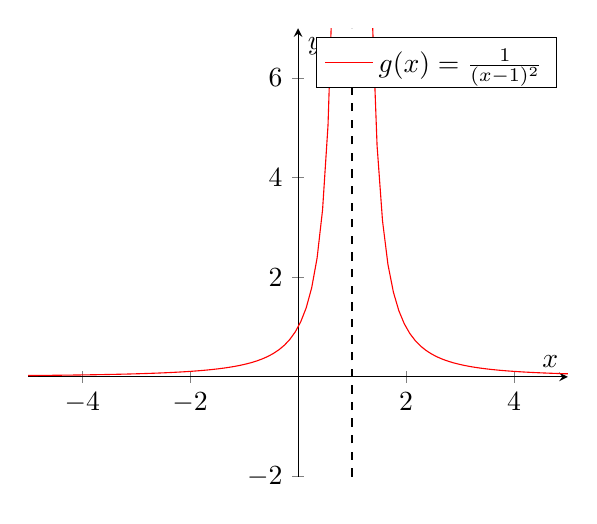
\begin{tikzpicture}
                    \begin{axis}[
                        axis lines = center,
                        xmin = -5,
                        xmax = 5,
                        ymin = -2,
                        ymax = 7,
                        xlabel={$x$},
                        ylabel={$y$},
                    ]
                    %g(x)
                    \addplot [
                        domain=-5:5,
                        samples=100,
                        color=red
                    ]
                    {(1)/((x-1)^2)};
                    \addlegendentry{$g(x)=\frac{1}{(x-1)^2}$}
                    %asymptote
                    \draw[
                        dashed
                    ]
                    (1,-2) -- (1,7);
                    \end{axis}
                \end{tikzpicture}
            \end{center}

            \noindent \color{purple} \textbf{The Rational Function Theorem:} \color{black} \\
            \noindent When $\lim_{x\to\pm\infty}\frac{P(x)}{Q(x)}=0$, $y=0$ is a horizontal asymptote
            of the graph of $y=\frac{P(x)}{Q(s)}$. \\
            When $\lim_{x\to\pm\infty}\frac{P(x)}{Q(x)}=\pm\infty$, the graph of $y=\frac{P(x)}{Q(x)}$
            has no horizontal asymptotes. \\
            When $\lim_{x\to\pm\infty}\frac{P(x)}{Q(x)}=\frac{a_n}{b_n}$, $y=\frac{a_n}{b_n}$ is a
            horizontal asymptote of the graph of $y=\frac{P(x)}{Q(x)}$.

        \pagebreak
        \subsection{The Squeeze Theorem}
            Functions $g$ and $h$ are strategically chosen to satisfy the conditions outlined in the
            definition. Notice how, in the figure after the definition, function $f$ is being
            "squeezed" between functions $g$ and $h$, hence the name. \\

            \noindent \color{purple} \textbf{The Squeeze Theorem:} \color{black} \\
            Assume that functions $f,g,h$ defined n $D\subseteq\mathbb{R}$ satisfy \\

            \begin{equation*}
                g(x)\leq f(x)\leq h(x),\forall x\in D
            \end{equation*}

            \noindent If $\lim_{x\to a}g(x)=\lim_{x\to a}h(x)=L$, then $\lim_{x\to a}f(x)=L$. \\

            \begin{center}
                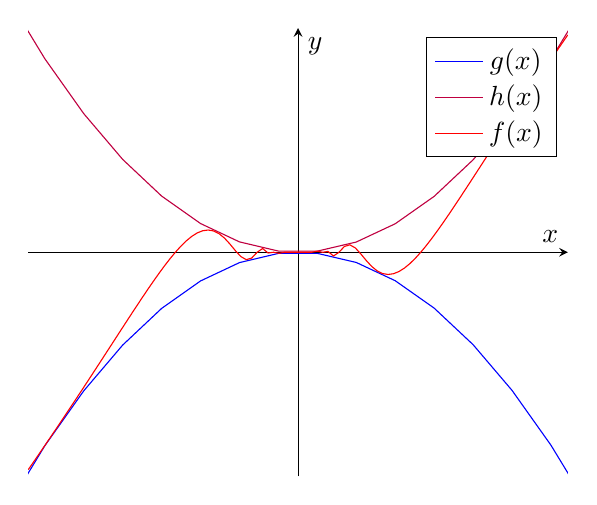
\begin{tikzpicture}
                    \begin{axis}[
                        axis lines = center,
                        xmin = -0.7,
                        xmax = 0.7,
                        ymin = -0.5,
                        ymax = 0.5,
                        xlabel={$x$},
                        ylabel={$y$},
                        \pgfplotset{ticks=none}
                    ]
                    %g(x)
                    \addplot [
                        samples=100,
                        color=blue
                    ]
                    {-x^2};
                    \addlegendentry{$g(x)$}
                    %h(x)
                    \addplot[
                        samples=100,
                        color=purple
                    ]
                    {x^2};
                    \addlegendentry{$h(x)$}
                    %f(x)
                    \addplot[
                        domain=-0.7:0.7,
                        samples=100,
                        color=red
                    ]
                    {x^2*sin(deg(1/\x))};
                    \addlegendentry{$f(x)$}
                    \end{axis}
                \end{tikzpicture}
            \end{center}

            \noindent \color{blue}
            \textit{Example 1: Given an infinite sequence $\{a_n\}$ that satisfies
            $\frac{2n^2-7}{4n+5}<a_n<\frac{3n^2+8}{6n-1}$ for all positive integers $n$, evaluate} \\

            \begin{equation}
                \lim_{n\to \infty}\frac{3na_n}{(n+1)^2}
            \end{equation}

            \color{black} \noindent We transform the middle term of the inequality to the desired
            expression through manipulating each side of the inequality. Then the inequality becomes \\

            \begin{equation*}
                \frac{3n}{(n+1)^2}\cdot\frac{2n^2-7}{4n+5}<\frac{3na_n}{(n+1)^2}<\frac{3n}{(n+1)^2}\cdot\frac{3n^2+8}{6n-1}
            \end{equation*}

            \noindent Now we can take the limits of the top and bottom functions. \\

            \begin{align*}
                \lim_{n\to \infty}\frac{3n(2n^2-7)}{(4n+5)(n+1)^2} &= \frac{3}{2} \\
                \lim_{n\to\infty}\frac{3n(3n^2+8)}{(6n-1)(n+1)^2} &= \frac{3}{2}
            \end{align*}

            \noindent Since the top and bottom functions are equal, we can conclude that \\

            \begin{equation*}
                \lim_{n\to\infty} \frac{3na_n}{(n+1)^2}=\frac{3}{2}
            \end{equation*}

            \noindent \color{blue} \textit{Example 2: Evaluate the limit} \\

            \begin{equation*}
                \lim_{n\to\infty}\sqrt[n]{3^n+\{2|\sin{(n^n)}\}^n}
            \end{equation*}

            \color{black} \noindent We can note that \\

            \begin{equation*}
                0\leq|\sin{(n^n)}|\leq1
            \end{equation*}

            \noindent Then we can write \\

            \begin{equation*}
                \sqrt[n]{3^n}\leq\sqrt[n]{3^n+\{2|\sin{(n^n)}\}^n}\leq\sqrt[n]{3^n+2^n}\leq\sqrt[n]{2\cdot3^n}
            \end{equation*}

            \noindent The left side reduces to 3, whereas the right side becomes \\

            \begin{equation*}
                \lim_{n\to\infty}\sqrt[n]{2\cdot3^n} = 3\lim_{n\to\infty}\sqrt[n]{2}=3
            \end{equation*}

            \noindent Thus we can conclude that \\

            \begin{equation*}
                \lim_{n\to\infty} \sqrt[n]{3^n+\{2|\sin{(n^n)}|\}^n} = 3
            \end{equation*}

            \noindent \color{blue} \textit{Example 3: Evaluate the limit} \\
            \begin{equation*}
                \lim_{x\to\infty}\frac{\sin{x}}{x}
            \end{equation*} \color{black}

            \noindent Since $\forall x,-1\leq\sin{x}\leq1$, it follows that if $x>0$ then
            $-\frac{1}{x}\leq\frac{\sin{x}}{x}\leq\frac{1}{x}$. As $x\rightarrow\infty$,
            $-\frac{1}{x}$ and $\frac{1}{x}$ both approach 0. Therefore, by the Squeeze Theorem,
            $\frac{\sin{x}}{x}$ also approaches 0. \\


        \subsection{Limit of a Quotient of Polynomials}
            For the function $f(x)=\frac{P(x)}{Q(x)}$, where $P(x)$ is a polynomial of degree $n$
            and $Q(x)$ is a polynomial of degree $m$, the following expressions hold. Let $a_n$
            and $b_n$ be the leading coefficients of $P(x)$ and $Q(x)$ respectively. Then \\

            \begin{equation*}
                \text{If $n>m$, then }\lim_{x\to\infty}f(x)=\infty\text{ and }
                \lim_{x\to-\infty}f(x)=-\infty
            \end{equation*}

            \begin{equation*}
                \text{If $n=m$, then }\lim_{x\to\pm\infty}f(x)=\frac{a_n}{b_m}
            \end{equation*}

            \begin{equation*}
                \text{If $n<m$, then }\lim_{x\to\pm\infty}f(x)=0
            \end{equation*}

            \noindent This method is a shortcut found through dividing each of the terms of $P(x)$
            and $Q(x)$ by the highest power of $x$ found in $f(x)$, then taking the individual limits
            of each separated term through basic limit properties. For example, see below. \\

            \noindent \color{blue} \textit{Example: Evaluate the limit} \color{black} \\

            \begin{align*}
                \lim_{x\to\infty}\frac{x^3-4x^2+7}{3-6x-2x^3} &=
                \lim_{x\to\infty}\frac{1-\frac{4}{x}+\frac{7}{x^3}}{\frac{3}{x^3}-\frac{6}{x^2}-2} \\
                &= \frac{\lim_{x\to\infty}(1)-\lim_{x\to\infty}\left(\frac{4}{x}\right)+\lim_{x\to\infty}\left(\frac{7}{x^3}\right)}{\lim_{x\to\infty\left(\frac{3}{x^3}\right)}-\lim_{x\to\infty}\left(\frac{6}{x^2}\right)-\lim_{x\to\infty}(2)} \\
                &= \frac{1-0+0}{0-0-2} \\
                &= -\frac{1}{2}
            \end{align*}

            \noindent Note that in this case, $n=m$, so $\frac{a_n}{b_n}\implies -\frac{1}{2}$.
            Since the properties described preceding this example can be observed in all quotients
            of polynomials, we can thus make generalizations as specificed above.


        \subsection{L'Hospital's Rule}
            \textbf{L'Hospital's} is a method of evaluating limits of indeterminate forms, learned
            after gaining knowledge of derivatives. \textbf{Indeterminate forms} are expressions i
            nvolving two functions whose limits cannot be determined solely from the limits of the
            individual functions. \\

            \noindent \color{purple} \textbf{The 7 Indeterminate Forms:} \\ \color{black}

            \begin{equation*}
                \frac{0}{0}, \frac{\infty}{\infty}, 0\cdot\infty, \infty-\infty, 0^0, 1^\infty, \infty^0
            \end{equation*}

            \noindent \color{purple} \textbf{L'Hospital's Rule:} \color{black} \\
            Suppose that we have either of the cases below \\

            \begin{equation*}
                \lim_{x\to a}\frac{f(x)}{g(x)}=\frac{0}{0}, \lim_{x\to a}\frac{f(x)}{g(x)}=\frac{\pm\infty}{\pm\infty}
            \end{equation*}

            \noindent where $a\in\mathbb{R}, \infty$ or $-\infty$. Then \\

            \begin{equation*}
                \lim_{x\to a}\frac{f(x)}{g(x)}=\lim_{x\to a}\frac{f'(x)}{g'(x)}
            \end{equation*}

            \noindent \color{blue} \textit{Example 1: Evaluate the limit} \\

            \begin{equation*}
                \lim_{t\to 1}\frac{5t^4-4t^2-1}{10-t-9t^3}
            \end{equation*}
            \color{black} We have an $\frac{0}{0}$ indeterminate form here, so we use L'Hospital's to get \\

            \begin{equation}
                \lim_{t\to 1}\frac{5t^4-4t^2-1}{10-t-9t^3}=\lim_{t\to 1}\frac{20t^3-8t}{-1-27t^2}
                =\frac{20-8}{-1-27}=-\frac{3}{7}
            \end{equation}

            \noindent \color{blue} \textit{Example 2: Evaluate the limit} \\

            \begin{equation*}
                \lim_{x\to-\infty}xe^x
            \end{equation*}
            \color{black} This expression is in the form $(\infty)(0)$, meaning we will have to write
            the expression as a quotient. We know that $\frac{1}{e^x}=e^{-x}$, so we can rewrite the
            limit as \\

            \begin{equation*}
                \lim_{x\to-\infty}xe^x=\lim_{x\to-\infty}\frac{x}{e^-x}=\lim_{x\to-\infty} \frac{1}{-e^-x}=0
            \end{equation*}

            \noindent \color{blue} \textit{Example 3: Evaluate the limit} \\

            \begin{equation*}
                \lim_{x\to\infty}x^{\frac{1}{x}}
            \end{equation*} \color{black}

            \noindent This limit is of the form $\infty^0$, so we have to rewrite this expression as a different
            limit. Let \\

            \begin{equation*}
                y &= x^{\frac{1}{x}} \\
            \end{equation*}

            \noindent Since \\

            \begin{equation*}
                e^{\ln{(y)}}=y
            \end{equation*}

            \noindent we can rewrite our limit as \\

            \begin{align*}
                \lim_{x\to\infty}x^{\frac{1}{x}} &= \lim_{x\to\infty} y \\
                &= \lim_{x\to\infty}e^{\ln{(y)}} \\
                &= e^{\lim_{x\to\infty}\ln{(y)}} \\
                &= e^0 \\
                &= 1
            \end{align*}

            \noindent L'Hospital's can help us prove \textbf{the basic trig limit}, useful for
            evaluating many trig limits. \\

            \begin{equation*}
                \lim_{\theta\to0}\frac{\sin{\theta}}{\theta}=1 \text{ if $\theta$ is measured in radians}
            \end{equation*}


        \pagebreak
        \subsection{Limit Strategies}
            KhanAcademy provides a convenient flowchart to illustrate a strategy to find limits: \\

            \begin{figure} [hbt!]
                \centering
                \includegraphics[scale=0.5]{Resources/Unit1Limits/limitstrat.png}
            \end{figure}

            \noindent \color{blue} \textit{Example 1:} \color{black} \\

            \begin{align*}
                \lim_{x\to 0}\frac{\sin{3x}}{x} &= \lim_{x\to0}\frac{3\sin{3x}}{3x} \\
                &= 3\lim_{x\to0}\frac{\sin{3x}}{3x} \\
                &= 3\cdot1\\
                &= 3
            \end{align*}

            \pagebreak
            \noindent \color{blue} \textit{Example 2:} \color{black} \\

            \begin{align*}
                \lim_{x\to0}\frac{\sin{2x}}{3x} &= \frac{1}{3}\lim_{x\to0}\frac{\sin{2x}}{x}\cdot\frac{2}{2} \\
                &= \frac{2}{3}\lim_{x\to0}\frac{\sin{2x}}{2x} \\
                &=\frac{2}{3}
            \end{align*}

            \noindent \color{blue} \textit{Example 3:} \color{black} \\

            \begin{align*}
                \lim_{x\to0}\frac{|x|}{x}
            \end{align*}

            \noindent Since $|x|=x$ if $x>0$ but $|x|=-x$ if $x<0$, $\lim_{x\to 0^+}\frac{|x|}{x}
            =\lim_{x\to0^+}\frac{x}{x}=1$, whereas
            $\lim_{x\to0^-}\frac{|x|}{x}=\lim_{x\to0^-}\frac{-x}{x}=-1$.
            Since the right and left hand limits are different, we can conclude that the
            limit does not exist.

            \noindent \color{blue} \textit{Example 4:} \color{black} \\
            \begin{align*}
                \lim_{x\to\infty}\arctan{(x^3-5x+6)} &= \arctan{(\lim_{x\to\infty}x^3-5x+6)} \\
                &= \arctan{(+\infty)} \\
                &= \frac{\pi}{2}
            \end{align*}

        \subsection{Limit Definition of $e$}
            The mathematical constant $e$ is defined by \\
            \begin{equation*}
                e=\lim_{n\to\infty}\left(1+\frac{1}{n}\right)^n
            \end{equation*}


        \subsection{Continuity and Discontinuity}
            A function $f(x)$ is \textbf{continuous} at $a$ if \\

            \begin{equation*}
                \lim_{x\to a}f(x)=f(a)
            \end{equation*}

            \noindent A function $f(x)$ is \textbf{continuous over the interval} $[a,b]$ if
            $\forall a\leq x\leq b$, $x$ is continuous. A function is \textbf{discontinuous} if it
            is not continuous. \\

            \noindent \color{purple} \textbf{Common Continuous Functions:} \color{black} \\
            $\bullet$ Polynomials are continuous everywhere at a real number. \\
            $\bullet$ Rational functions are continuous at each point in their domain except where
            $Q(x)=0$. \\
            $\bullet$ The absolute value function is continuous everywhere. \\
            $\bullet$ The trigonometric, inverse trigonometric, exponential, and logarithmic functions
            are continuous everywhere. \\
            $\bullet$ Irrational functions in the form $\sqrt[n]{x}$, where $n\geq 2$, are continuous
            everywhere for which $\sqrt[n]{x}$ is defined. \\
            $\bullet$ The greatest-integer function is discontinuous at each integer. \\

            \noindent \color{purple} \textbf{Types of Discontinuities:} \\
            \noindent \textbf{Jump Discontinuity:} \color{black} \\
            In a jump discontinuity, the left and right-hand limits exist, but are different.
            For example, the graph of $y=f(x)$ below has a jump discontinuity at $x=1$. \\

            \begin{center}
                \begin{tikzpicture}
                    \begin{axis}[
                        axis lines = center,
                        axis equal image,
                        xmin = -5,
                        xmax = 5,
                        ymin = -5,
                        ymax = 5,
                    ]
                    %f(x), x<1
                    \addplot [
                        domain = -5:1,
                        samples = 100,
                        color = red
                    ]
                    {-x/3};
                    \addlegendentry{$y=f(x)$}
                    %f(x), x>1
                    \addplot[
                        domain = 1:5,
                        samples = 100,
                        color = red
                    ]
                    {-((x-2)^2)/(2)+3.5};
                    %undefined circle at x = 1
                    \path[
                        draw = black,
                        fill = white,
                    ]
                    (1,3) circle [radius = 0.1];
                    %defined circle at x = 1
                    \fill[black] (1,-0.3333) circle [radius = 0.1];
                    \end{axis}
                \end{tikzpicture}
            \end{center}

            \noindent \color{purple} \textbf{Removable Discontinuity:} \color{black} \\
            A function $f(x)$ has a removable discontinuity at $x=a$ if $\lim_{x\to a}f(x)$ exists,
            but either $f(a)$ does not exist or the value of $f(a)\not=\lim_{x\to a}f(x)$.
            A function with a removable discontinuity at $a$ may or may not be defined at $a$.
            For example, the graph of $y=g(x)$ below has a removable discontinuity at $x=1$.
            In this case, $g(1)=3$ instead of the limit value $\lim_{x\to1}g(x)=\sin{(1)}$. \\

            \begin{center}
                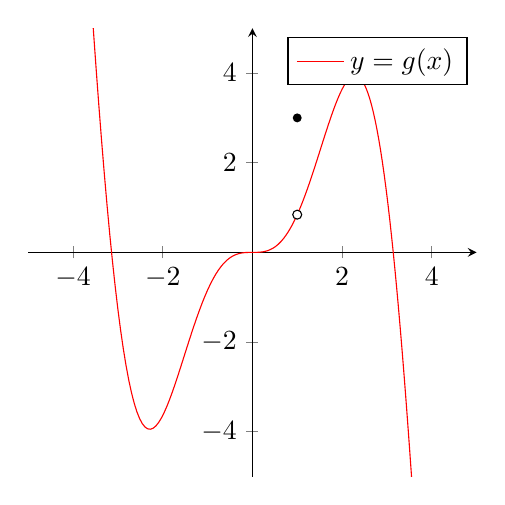
\begin{tikzpicture}
                    \begin{axis}[
                        axis lines = center,
                        axis equal image,
                        xmin = -5,
                        xmax = 5,
                        ymin = -5,
                        ymax = 5,
                    ]
                    %g(x), x<1
                    \addplot [
                        domain = -5:1,
                        samples = 100,
                        color = red
                    ]
                    {sin(deg(x))*x^2};
                    \addlegendentry{$y=g(x)$}
                    %g(x), x>1
                    \addplot[
                        domain = 1:5,
                        samples = 100,
                        color = red
                    ]
                    {sin(deg(x))*x^2};
                    %undefined circle at x = 1
                    \path[
                        draw = black,
                        fill = white,
                    ]
                    (1,0.84147) circle [radius = 0.1];
                    %defined circle at x = 1
                    \fill[black] (1,3) circle [radius = 0.1];
                    \end{axis}
                \end{tikzpicture}
            \end{center}

            \noindent \color{purple} \textbf{Infinite Discontinuities:} \color{black} \\
            Infinite discontinuities always occur at vertical asymptotes. There may be a vertical
            asymptote at either one or both sides of the function. An example of an infinite
            discontinuity is given below, where $y=h(x)$. \\

            \begin{center}
                \begin{tikzpicture}
                    \begin{axis}[
                        axis lines = center,
                        axis equal image,
                        xmin = -5,
                        xmax = 5,
                        ymin = -3,
                        ymax = 7,
                    ]
                    %h(x)
                    \addplot [
                        samples = 100,
                        color = red
                    ]
                    {1/((x-1)^2)};
                    \addlegendentry{$y=h(x)$}
                    %asymptote
                    \draw[
                        dashed
                    ]
                    (1,-3) -- (1,7);
                    \end{axis}
                \end{tikzpicture}
            \end{center}

            \noindent Here is an example of an \color{purple} \textbf{Infinite Oscillation Discontinuity}.
            \color{black} \\

            \begin{center}
                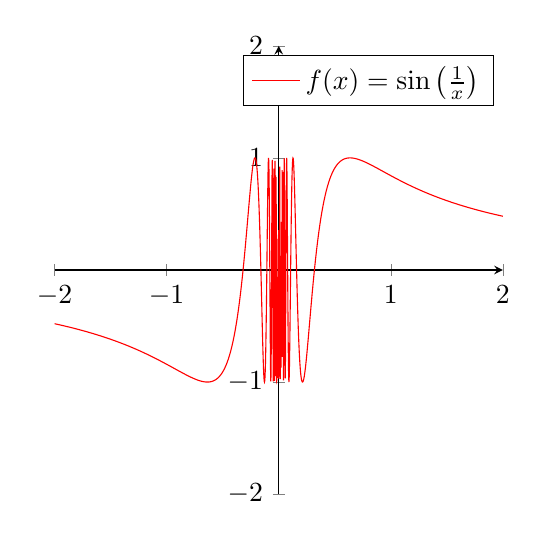
\begin{tikzpicture}
                    \begin{axis}[
                        axis lines = center,
                        axis equal image,
                        xmin = -2,
                        xmax = 2,
                        ymin = -2,
                        ymax = 2,
                    ]
                    %f(x)
                    \addplot [
                        samples = 5000,
                        color = red
                    ]
                    {sin(deg(1/x))};
                    \addlegendentry{$f(x)=\sin{\left(\frac{1}{x}\right)}$}
                    \end{axis}
                \end{tikzpicture}
            \end{center}

            \noindent \color{purple} \textbf{Essential Discontinuities} \color{black} are discontinuities
            that at which the limit of the function does not exist. Jump and infinite discontinuities
            are essential discontinuities. \\\\

            Below is a general example about continuity and discontinuity. \\
            \color{blue} \textit{Example: Is} \\

            \begin{equation*}
                f(x)=\begin{cases}
                {
                x^2+2 & x\leq 1 \\
                4 & x > 1
                }
                \end{cases}
            \end{equation*}

            \noindent continuous at $x=1$? \color{black} \\
            Since $\lim_{x\to 1^-}f(x)=3\not=\lim_{x\to 1^+}f(x)=4$.

        \subsection{The Extreme Value Theorem}

            This theorem is best learnt after derivatives. \\
            \color{purple} \textbf{The Extreme Value Theorem} \color{black} \\
            If real numbers $a$ and $b$ satisfy $a<b$ and a function $f$ is continuous on $[a,b]$,
            then $f$ attains a maximum and minimum value on $[a,b]$. \\

            \noindent \color{blue} \textit{Example: Find the maximum and minimum values of the
            function $f(x)=x^3-\frac{9}{2}x^2-12x+20$ on the interval $[-2,6]$}. \color{black} \\
            $f(x)$ is differentiable, hence continuous on the closed and bounded interval. Having
            satisfied the preconditions, we can apply the EVT to this context. Taking the first
            derivative of $f(x)$, we get \\

            \begin{align*}
                f'(x) &= 3x^2 -9x -12 \\
                &= 3(x^2-3x-4)
            \end{align*}

            \noindent Setting $f'(x)=0$ and solving, we find that the critical points are $x=-1,4$
            which by the first derivative test gives the relative extrema $y=26.5,-36$, respectively.
            Computing the endpoints, we have $f(-2)=18$ and $f(6)=2$. Hence, the minimum value of $f$
            on $[-2,6]$ is -36 and the maximum value is 26.5.


        \subsection{The Intermediate Value Theorem}
            \color{purple} \textbf{The Intermediate Value Theorem:} \color{black} \\
            If a function $f$ is continuous on the closed interval $[a,b]$, and $M$ is a number such
            that $f(a)\leq M\leq f(b)$, then there is at least one number $c$ such that $f(c)=M$. \\

            \noindent \color{blue} \textit{Example: Does a $x$ exist for some $x\in[0,2]$ such that
            the function $f(x)=x^2+\cos{(\pi x)}=4$?} \color{black} \\

            \begin{align*}
                f(0) = 0^2 + \cos{0} = 1 \\
                f(2) = 2^2 + \cos{2\pi} = 5
            \end{align*}

            \noindent Since $f(0)=1<4<5=f(2)$ and $f$ is continuous, the IVT implies that $f(x)=4$
            for some $x\in[0,2]$.


        \subsection{The Continuous Functions Theorem}
            \color{purple} \textbf{The Continuous Functions Theorem:} \color{black} \\
            If functions $f$ and $g$ are both continuous at $x=c$, then the following functions are
            also continuous: \\

            \begin{tabular}{cc}
                Constant Multiples: & $k\cdot f(x)$ for any real number $k$ \\
                Sums: & $f(x)+g(x)$ \\
                Differences: & $f(x)-g(x)$ \\
                Products: & $f(x)\cdot g(x)$ \\
                Quotients: & $\frac{f(x)}{g(x)}, g(c)\not=0$
            \end{tabular}


        \subsection{The Composition of Continuous Functions Theorem}
            \color{purple} \textbf{The Composition of Continuous Functions Theorem:} \color{black} \\
            If the function $g$ is continuous at $x=c$ and the function $f$ is continuous at $x=g(c)$,
            then the composite function $(f\circ g)(x)$ is continuous at $x=c$.

    \pagebreak
%%%-------------------------------------------NEW SECTION--------------------------------------%%%

    \section{Differentiation}

        \subsection{Rates of Change and Derivatives}
            An \textbf{average rate of change} describes the overall
            $\frac{\text{rise}}{\text{run}}$-value over an interval $[a,b]$. Geometrically,
            this can be represented by the slope of a secant line through $f(a)$ and $f(b)$ of a
            function $f(x)$. In the graph below, the average rate of change between $x=0$ and
            $x=2$ is given by \\

            \begin{equation*}
                m_{\text{avg}} = \frac{f(b)-f(a)}{b-a} = \frac{4-0}{2-0} = 2
            \end{equation*}

            \begin{center}
                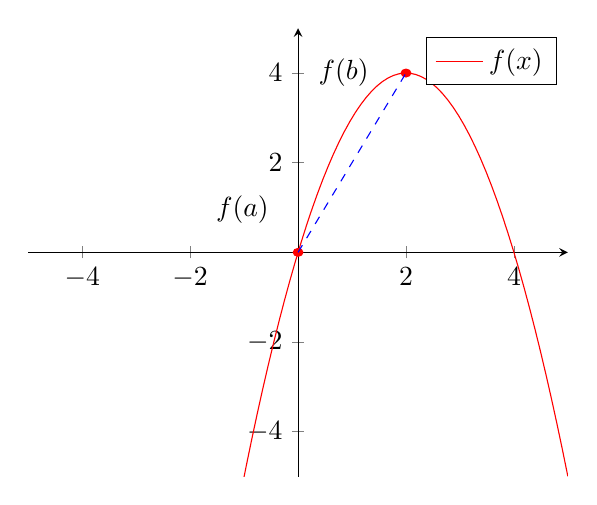
\begin{tikzpicture}
                    \begin{axis} [
                        axis lines = center,
                        xmin = -5,
                        xmax = 5,
                        ymin = -5,
                        ymax = 5
                    ]
                    %f(x)
                    \addplot[
                        color = red,
                        samples = 100,
                    ]
                    {-(x-2)^2+4};
                    \addlegendentry{$f(x)$}
                    %f(a)
                    \fill[red] (0,0) circle [radius = 0.1];
                    \node [
                        above left = 10pt of {(0,0)}
                    ]
                    {$f(a)$};
                    %f(b)
                    \fill[red] (2,4) circle [radius = 0.1];
                    \node[
                        left = 10pt of
                        {(2,4)}
                    ]
                    {$f(b)$};
                    %secant
                    \draw [
                        dashed,
                        color = blue
                    ]
                    (0,0) -- (2,4);
                    \end{axis}
                \end{tikzpicture}
            \end{center}

            \noindent A derivative is an \textbf{instantaneous rate of change}, or the slope of the
            tangent to a function at a particular point, $a$. Derivatives are always taken
            \textit{with respect} to a variable. For example, a derivative representing the
            instantaneous rate of change between distance and time is a derivative of distance
            with respect to time, the independent variable. For reference, the derivative of a
            function $f(x)$ at $x=1$ is shown in the graph below. \\

            \begin{center}
                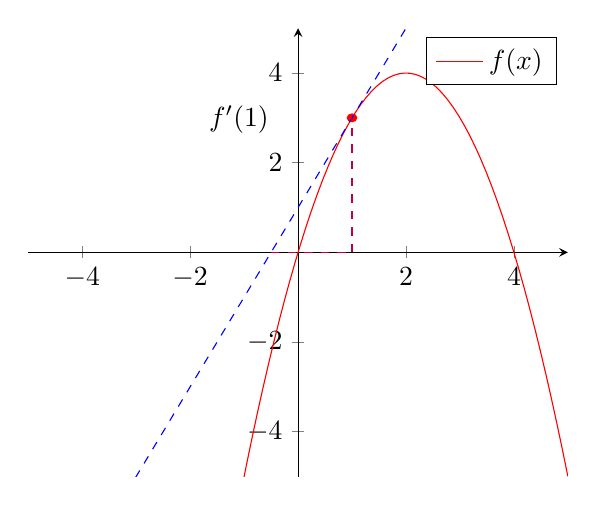
\begin{tikzpicture}
                    \begin{axis} [
                        axis lines = center,
                        xmin = -5,
                        xmax = 5,
                        ymin = -5,
                        ymax = 5
                    ]
                    %f(x)
                    \addplot[
                        color = red,
                        samples = 100,
                    ]
                    {-(x-2)^2+4};
                    \addlegendentry{$f(x)$}
                    %f(1)
                    \fill[red] (1,3) circle [radius = 0.1];
                    \node [
                        above left = 10pt of {(0,2)}
                    ]
                    {$f'(1)$};
                    %tangent
                    \draw [
                        dashed,
                        color = blue
                    ]
                    (5,11) -- (-5,-9);
                    %rise
                    \draw[
                        dashed,
                        color = purple
                    ]
                    (1,0) -- (1,3);
                    %run
                    \draw[
                        dashed,
                        color = purple
                    ]
                    (-0.5,0) -- (1,0);
                    \end{axis}
                \end{tikzpicture}
            \end{center}

            \noindent Since the derivative is an instantaneous rate of change, we can define the
            derivative as below. \\
            \color{purple} \textbf{$1^{st}$ Limit Definition of the Derivative} \color{black} \\
            The derivative of $f(x)$ with respect to $x$ is the function $f'(x)$, defined as \\

            \begin{equation*}
                f'(x) = \lim_{x\to a} \frac{f(x)-f(a)}{x-a}
            \end{equation*}

            \noindent Then, if we let $x=a+h$ and change the variable of inspection from $a$ to $x$,
            we can realize the most commonly used definition of the derivative, given below. This
            definition is preferred to the above definition, as finding the derivative only requires
            one value of $x$, rather than 2.  \\
            \color{purple} \textbf{$2^{nd}$ Limit Definition of the Derivative} \color{black} \\
            The derivative of $f(x)$ with respect to $x$ is the function $f'(x)$, defined as \\

            \begin{equation*}
                f'(x) = \lim_{h\to 0} \frac{f(a+h)-f(x)}{h}
            \end{equation*}

            \noindent The expression consisting the right side of the equation above is known as the
            \textbf{difference quotient}. \\

            \noindent A function is $f(x)$ is \textbf{differentiable} at $x=a
            $ if $f'(a)$ exists. Since derivatives are defined by limits, for a derivative to exist,
            its limit must also exist. Hence, \\

            \begin{equation*}
                \text{If $f(x)$ is differentiable at $x=a$ then $f(x)$ is continuous at $x=a$}
            \end{equation*}

            \noindent By this, we can also say that differentiability implies continuity. It is
            important to note that its converse is not always true, as not all continuous functions
            are differentiable. \\


            \noindent A few examples of contexts where a derivative may not exist are at vertical
            tangents, corners, and cusps. Take, for example, the graph below, which does not have a
            derivative at $x=0$ since the respective slopes immediately right and left of $x=0$ are
            different. \\

            \begin{center}
                \begin{tikzpicture}
                    \begin{axis}[
                        axis lines = center,
                        axis equal image
                    ]
                    %f(x)
                    \addplot [
                        samples = 50,
                        color = red,
                    ]
                    {abs(x)};
                    \addlegendentry{$f(x)=|x|$}
                    \end{axis}
                \end{tikzpicture}
            \end{center}

            \noindent \color{purple} \textbf{Derivative Notations:} \\
            \noindent \textbf{Leibniz's Notation:} \color{black} \\
            The Leibniz notation is popular throughout mathematics, most commonly used when the
            equation $y=f(x)$ is regarded as a functional relationship between dependent and
            independent variables $y$ and $x$. Leibniz's notation makes this relationship explicit
            by representing the derivative as \\

            \begin{equation*}
                \frac{dy}{dx}=\frac{d}{dx}y
            \end{equation*}

            \noindent The Leibniz notation is also called \textbf{differential notation}, where
            $dy$ and $dx$ are \textbf{differentials}. Where the function $y=f(x)$, we can write \\

            \begin{equation*}
                \frac{df}{dx}(x)=\frac{df(x)}{dx}=\frac{d}{dx}f(x)
            \end{equation*}

            \noindent A \textbf{differential equation} is an equation relating one or more functions
            and their derivatives. As long as the precondition ($f(x)$ is satisfied), a function can
            be differentiated indefinite times. For example, in physics, acceleration is the
            derivative of velocity, the derivative of position. The \textbf{order} of a differential
            equation is the highest derivative of said equation. Higher-order derivatives can be
            written in the Leibniz's notation as \\

            \begin{equation*}
                \frac{d^2y}{dx^2}, \frac{dy^3}{dx^3}, \frac{dy^4}{dx^4},\dots,\frac{d^ny}{dx^n}
            \end{equation*}

            \noindent With Leibniz's notation, the value of a derivative at a particular point, $a$,
            can be expressed as \\

            \begin{equation*}
                \frac{dy}{dx}\Bigr|_{x=a}
            \end{equation*}

            \noindent This notation is particularly useful in expressing partial derivatives
            (covered later) and making the chain rule intuitive: \\

            \begin{equation*}
                \frac{dy}{dx} = \frac{dy}{du}\cdot\frac{du}{dx}
            \end{equation*}

            \noindent \color{purple} \textbf{Lagrange's Notation:} \color{black} \\
            In Lagrange's notation, each prime mark denotes a derivative. For higher-order derivatives,
            the order is enclosed by parantheses in front and above the function. \\

            \begin{equation*}
                f'(x), f''(x), f'''(x), f^{(4)}(x),f^{(5)}(x),f^{(6)}(x),f^{(n)}(n)
            \end{equation*}

            \noindent \color{purple} \textbf{Newton's Notation:} \color{black} \\

            This notation is often applied to physics contexts, where time ($t$) is the independent
            variable. The number of dots over the dependent variable represent the order the
            derivative is in. If $y$ is a function of $t$, then the first $n$ derivatives of
            the function are as below. \\

            \begin{equation*}
                \dot{y}, \ddot{y}, \dddot{y}, _{\dot{y}}^4, _{\dot{y}}^5, _{\dot{y}}^n
            \end{equation*}

            \noindent \color{purple} \textbf{Euler's Notation:} \color{black} \\
            This notation is quite inconvenient, as it leaves the variable being differentiated with
            respect to entirely implicit. However, we can modify the notation to explicitly write
            said variable. This notation is defined by \\

            \begin{equation*}
                (Df)(x) = \frac{df(x)}{dx}
            \end{equation*}

            \pagebreak
            \noindent Higher-order Derivatives are expressed by \\

            \begin{equation*}
                D^2f=D^2_xf, D^3f=D^3_xf, D^nf=D^n_xf
            \end{equation*}

            \noindent \color{blue} \textit{Example 1: Find the derivative, $g'(t)$, given the function} \\

            \begin{equation}
                g(t) = \frac{t}{t+1}
            \end{equation} \color{black}

            \begin{align*}
                g'(t) &= \lim_{h\to 0} \frac{g(t+h)-g(t)}{h} \\
                &= \lim_{h\to 0} \frac{1}{h}\left(\frac{t+h}{t+h+1}-\frac{t}{t+1}\right) \\
                &= \lim_{h\to 0}\left(\frac{(t+h)(t+1)-t(t+h+1)}{(t+h+1)(t+1)}\right) \\
                &= \lim_{h\to 0} \frac{1}{h}\left(\frac{t^2+t+th+h-(t^2+th+t)}{(t+h+1)(t+1)}\right) \\
                &= \lim_{h\to 0} \frac{1}{h} \left(\frac{h}{(t+h+1)(t+1)}\right) \\
                &= \frac{1}{(t+1)(t+1)} \\
                g'(t) &= \frac{1}{(t+1)^2}
            \end{align*}

            \noindent \color{blue} \textit{Example 2: Find the derivative, $f'(x)$, of } \\

            \begin{equation*}
                f(x) = 2x^2-16x+35
            \end{equation*} \color{black}

            \begin{align*}
                f'(x) &= \lim_{h\to 0} \frac{2(x+h)^2-16(x+h)+35-(2x^2-16x+35)}{h} \\
                &= \lim_{h\to 0} \frac{4xh+2h^2-16h}{h} \\
                &= \lim_{h\to 0} (4x+2h-16) \\
                f'(x) &= 4x-16
            \end{align*}


        \subsection{Basic Derivative Rules}
            \begin{center}
                \begin{tabular}{|c|c|}
                    \hline
                    $\frac{d}{dx}a = 0$ & \textbf{Constant} \\
                    \hline
                    $\frac{d}{dx}au = a\frac{du}{dx}$ & \textbf{Constant Multiple} \\
                    \hline
                    $\frac{d}{dx}x^n=nx^{n-1}$ & \color{purple} \textbf{The Power Rule} \color{black} \\
                    \hline
                    $\frac{d}{dx}(u\pm v) = \frac{d}{dx}u \pm \frac{d}{dx}v$ & \textbf{Sum/Difference}\\
                    \hline
                    $\frac{d}{dx}(uv) = u\frac{dv}{dx}+v\frac{du}{dx}$ & \color{purple}
                    \textbf{The Product Rule} \color{black} \\
                    \hline
                    $\frac{d}{dx}\left(\frac{u}{v}\right)=\frac{v\frac{du}{dx}-u\frac{dv}{dx}}{v^2},
                    v\not = 0$ & \color{purple} \textbf{The Quotient Rule} \color{black} \\
                    \hline
                    $[f^{-1}]'(b)=\frac{1}{f'(a)}$ & \textbf{Inverse Functions} \\
                    \hline
                    $\frac{d}{dx}[f^{-1}(x)]=\frac{1}{f'(f^{-1}(x))}=\frac{1}{\frac{dy}{dx}}$ &
                    \textbf{Alternate Inverse Functions} \\
                    \hline
                    $\frac{d(1/f)}{dx}=-\frac{1}{f^2}\frac{df}{dx}$ & \textbf{Reciprocal} \\
                    \hline
                \end{tabular}
            \end{center}


        \subsection{Derivatives of Exponential and Logarithmic Functions}
            \begin{center}
                \begin{tabular}{|c|c|}
                    \hline
                    $\frac{d}{dx}e^x=e^x$ & \textbf{Natural Exponent} \\
                    \hline
                    $\frac{d}{dx}\ln{x}=\frac{1}{x}$ & \textbf{Natural Logarithm} \\
                    \hline
                    $\frac{d}{dx}a^x=a^x\ln{a}$ & \textbf{Exponent} \\
                    \hline
                    $\frac{d}{dx}\log_b{x}=\frac{1}{x\ln{b}}$ & \textbf{Logarithm} \\
                    \hline
                    $\frac{d}{dx}x^x=x^x(1+\ln{x})$ & \\
                    \hline
                \end{tabular}
            \end{center}


        \pagebreak
        \subsection{Derivatives of the Trigonometric Functions}
            The derivatives of $\sin{x}$ and $\cos{x}$ help us derive the others through applying
            the quotient and reciprocal differentiation rules. \\

            \begin{center}
                \begin{tabular}{|c|}
                    \hline
                    $\frac{d}{dx}\sin{x}=\cos{x}$ \\
                    \hline
                    $\frac{d}{dx}\cos{x}=-\sin{x}$ \\
                    \hline
                    $\frac{d}{dx}\tan{x}=\sec^2{x}$ \\
                    \hline
                    $\frac{d}{dx}\csc{x}=-\cot{x}\csc{x}$ \\
                    \hline
                    $\frac{d}{dx}\sec{x}=\tan{x}\sec{x}$ \\
                    \hline
                    $\frac{d}{dx}\cot{x}=-\csc^2{x}$ \\
                    \hline
                \end{tabular}
            \end{center}

            \noindent The derivatives of the inverse trigonometric functions can be derived through
            applying the inverse differentiation rule. \\

            \begin{center}
                \begin{tabular}{|c|}
                    \hline
                    $\frac{d}{dx}\arcsin{x} = \frac{1}{\sqrt{1-x^2}}$ \\
                    \hline
                    $\frac{d}{dx}\arccos{x} = -\frac{1}{\sqrt{1-x^2}}$ \\
                    \hline
                    $\frac{d}{dx}\arctan{x} = \frac{1}{1+x^2}$ \\
                    \hline
                    $\frac{d}{dx}\arccsc{x} = -\frac{1}{|x|\sqrt{x^2-1}}$ \\
                    \hline
                    $\frac{d}{dx}\arcsec{x} = \frac{1}{|x|\sqrt{x^2-1}}$ \\
                    \hline
                    $\frac{d}{dx}\arccot{x} = -\frac{1}{1+x^2}$ \\
                    \hline
                \end{tabular}
            \end{center}


            \noindent \color{purple} \textbf{Derivation of the Inverse Sine Derivative:} \color{black} \\
            \begin{align*}
                \frac{d(\arcsin{x})}{dx} &= \frac{1}{\frac{d(\sin{y})}{dy}} \\
                &= \frac{1}{\cos{y}} \\
            \end{align*}
            \noindent From the Pythagorean Identity, \\
            \begin{align*}
                \cos^2{y} + \sin^2{y} &= 1 \\
                \cos^2{y} &= 1 - \sin^2{y} \\
                \cos{y} &= \sqrt{1-\sin^2{y}}
            \end{align*}
            \noindent Substituting this back into the original equation, we get \\
            \begin{align*}
                \frac{d(\arcsin{x})}{dx} &= \frac{1}{\sqrt{1-\sin^2{y}}}
            \end{align*}
            \noindent By the definition of the inverse sine function, we can express the equation as \\
            \begin{align*}
                \frac{d}{dx}\arcsin{x} &= \frac{1}{\sqrt{1-x^2}}
            \end{align*}

            \noindent \color{purple} \textbf{Derivation of the Inverse Cosine Derivative} \color{black} \\
            The derivatives of the inverse trigonometric functions are the \textit{negatives} of the
            derivatives of their cofunctions. This is because \\

            \begin{align*}
                \arccos{x} &= \frac{\pi}{2} - \arcsin{x} \\
                \frac{d}{dx}\arccos{x} &= -\frac{d}{dx}\arcsin{x} \\
                &= -\frac{1}{\sqrt{1-x^2}}
            \end{align*}

            \noindent \color{purple} \textbf{Derivation of the Inverse Tangent Derivative} \color{black} \\

            \begin{align*}
                \frac{d}{dx}\arctan{x} &= \frac{1}{\frac{d(\tan{y})}{dy}} \\
                &= \frac{1}{\sec^2{y}} \\
                &= \frac{1}{1+\tan^2{y}} \\
                &= \frac{1}{1+x^2}
            \end{align*}

        \pagebreak
        \subsection{The Chain Rule}
            The Chain Rule is incredibly useful for finding the derivative of composite functions.
            If $y=f(u)$ and $u=g(x)$ then \\

            \begin{align*}
                (f(g(x)))' &= f'(g(x)) \cdot g'(x) \\
                &= f'(u) \cdot g'(x) \\
                \frac{dy}{dx} &= \frac{dy}{du} \cdot \frac{du}{dx}
            \end{align*}

            \noindent \color{blue} \textit{Example 1:} \color{black} \\

            \begin{align*}
                f(x) &= \sqrt{5x-8} \\
            \end{align*}

            \noindent We let the inside function be expressed as $u=5x-8$. Then \\

            \begin{align*}
                f'(x) &= \frac{du}{dx}u^{\frac{1}{2}}\cdot\frac{dy}{du}(5x-8) \\
                &= \frac{1}{2\sqrt{u}}\cdot 5 \\
                &= \frac{5}{2\sqrt{5x-8}}
            \end{align*}

            \noindent \color{blue} \textit{Example 2:} \color{black} \\
            \noindent Let $u=\cos{t}$ and $v=t^4$

            \begin{align*}
                g(t) &= \cos^4{t} + \cos{(t^4)} \\
                g'(t) &= \frac{d(u^4)}{du} \cdot \frac{d}{dt}\cos{t}
                +
                \frac{d(t^4)}{dt} \cdot \frac{d(\cos{v})}{dv} \\
                &= 4u^3(-\sin{t}) + 4t^3(-\sin{v}) \\
                &= -4\cos^3{t}\sin{t} - 4t^3\sin{(t^4)}
            \end{align*}

        \subsection{Implicit Differentiation}
            \color{purple} \textbf{Implicit Differentiation} \color{black} is an approach to
            differentiating a function that may not be in the explicit form, $y=f(x)$. It
            considers all other variables as functions of one of its variables, then uses the
            chain rule to find the derivative. \\

            \noindent \color{blue} \textit{Example 1: Given $x^2+x+y^2=15$, what is $\frac{dy}{dx}$
            at the point $(2,3)$?} \color{black} \\

            \begin{align*}
                \frac{dy}{dx}(x^2+x+y^2) &= \frac{dy}{dx}15 \\
                2x + 1 + 2y\left(\frac{dy}{dx}\right) &= 0 \\
                \frac{dy}{dx} &= -\frac{2x+1}{2y} \\
                \frac{dy}{dx}\Bigr|_{(2,3)} &= -\frac{2(2)+1}{2(3)} \\
                &= -\frac{5}{6}
            \end{align*}

            \noindent \color{blue} \textit{Example 2: Find the derivative of
            $\ln{y}+e^y=\sin{y^2}-3\cos{x}$} \color{black} \\

            \begin{align*}
                \frac{dy}{dx}\ln{y} + \frac{dy}{dx}e^y &= \frac{d}{dx}\sin{y^2}-\frac{d}{dx}3\cos{x} \\
                \frac{d}{dy}\ln{y}\cdot\frac{dy}{dx}+\frac{d}{dy}e^y\cdot\frac{dy}{dx}
                &= \frac{d}{dy}\sin{y^2}\cdot\frac{dy}{dx}+3\sin{x} \\
                \frac{dy}{dx}\left(\frac{1}{y}+e^y-2y\cos{y^2}\right) &= 3\sin{x} \\
                \frac{dy}{dx} &= \frac{3\sin{x}}{\frac{1}{y}+e^y-2y\cos{y^2}}
            \end{align*}

            \noindent \color{blue} \textit{Example 3: Find $\frac{dy}{dx}$ if $y^2 &= x^2 + \sin{(xy)}$}
            \color{black} \\

            \begin{align*}
                \frac{d}{dx}(y^2) &= \frac{d}{dx}(x^2) + \frac{d}{dx}(\sin{(xy)} \\
                2y\frac{d}{dx} &= 2x + (\cos{(xy)})\left(y+x\frac{d}{dx}\right) \\
                (2y-x\cos{(xy)})\frac{d}{dx} &= 2x + y\cos{(xy)} \\
                \frac{dy}{dx} &= \frac{2x+y\cos{(xy)}}{2y-x\cos{(xy)}}
            \end{align*}


        \subsection{Logarithmic Differentiation}
            This method of finding derivatives uses the basic properties of logarithms outside
            of calculus to simply a function prior to differentiating it. \\

            \noindent \color{blue} \textit{Example 1:} \color{black} \\

            \begin{align*}
                y &= \frac{x^5}{(1-10x)\sqrt{x^2+2}} \\
                \ln{y} &= \ln{\left(\frac{x^5}{(1-10x)\sqrt{x^2+2}}\right)} \\
                &= \ln{(x^5)} - \ln{\left((1-10x)\sqrt{x^2+2}\right)} \\
                &= \ln{(x^5)} - \ln{(1-10x)} - \ln{(\sqrt{x^2+2})}
            \end{align*}

            \noindent By Implicit Differentiation, \\

            \begin{align*}
                \fra{y'}{y} &= \frac{5x^4}{x^5}- \frac{-10}{1-10x} - \frac{\frac{1}{2}(x^2+2)^{-\frac{1}{2}}(2x)}{(x^2+2)^{\frac{1}{2}}} \\
                &= \frac{5}{x} + \frac{10}{1-10x} - \frac{x}{x^2+2} \\
                \frac{dy}{dx} &= \frac{x^5}{(1-10x)\sqrt{x^2+2}}\left(\frac{5}{x}+\frac{10}{1-10x}-\frac{x}{x^2+2}\right)
            \end{align*}

            \noindent \color{blue} \textit{Example 2:} \color{black} \\

            \begin{align*}
                y &= \frac{x+3}{(x+4)^3} \\
                \ln{y} &= \ln{\left(\frac{x+3}{(x+4)^3}\right)} \\
                &= \ln{(x+3)} - \ln{(x+4)^3} \\
                &= \ln{(x+3)}  - 3\ln{(x+4)} \\
                \frac{1}{y}\cdot\frac{dy}{dx} &= \frac{1}{x+3}-3\cdot\frac{1}{x+4} \\
                &= \frac{1}{x+3}-\frac{3}{x+4} \\
                \frac{dy}{dx} &= y\left(\frac{1}{x+3}-\frac{3}{x+4}\right)
            \end{align*}


        \subsection{Derivatives of Parametric Functions}
            If $x=f(t)$ and $y=g(t)$ are differentiable functions of parameter $t$, then \\

            \begin{equation*}
                \frac{dy}{dx} = \frac{\frac{dy}{dt}}{\frac{dx}{dt}}
            \end{equation*}

            \noindent and

            \begin{equation*}
                \frac{d^2y}{dx^2} = \frac{d}{dx}\left(\frac{dy}{dx}\right)
                = \frac{\frac{d}{dt}\left(\frac{dy}{dx}\right)}{\frac{dx}{dt}}
            \end{equation*}

            \noindent \color{blue} \textit{Example: If $x=2\sin{\theta}$ and $y=\cos{2\theta}$,
            find $\frac{d^2y}{dx^2}$} \color{black} \\

            \begin{align*}
                \frac{dy}{dx} &= \frac{\frac{dy}{d\theta}}{\frac{dx}{d\theta}} \\
                &= \frac{-2\sin{2\theta}}{2\cos{\theta}} \\
                &= -\frac{2\sin\theta\cos\theta}{\cos\theta} \\
                &= -2\sin\theta
            \end{align*}

            \begin{align*}
                \frac{d^2y}{dx^2} &= \frac{\frac{d}{d\theta}\left(\frac{dy}{dx}\right)}{\frac{dx}{d\theta}} \\
                &= \frac{-2\cos\theta}{2\cos\theta} \\
                &= -1
            \end{align*}



        \subsection{Derivatives of Polar Functions}
            We know that $x=r\cos\theta$ and $y=r\sin\theta$. Then, by using the parametric derivative
            formula, we can determine the rule for differentiating polar functions. \\

            \begin{align*}
                \frac{dy}{dx} &= \frac{\frac{dy}{d\theta}}{\frac{dx}{d\theta}} \\
                &= \frac{f'(\theta)\sin\theta+f(\theta)\cos\theta}{f'(\theta)\cos\theta-f(\theta)\sin\theta} \\
                &= \frac{r'\sin\theta+r\cos\theta}{r'\cos\theta-r\sin\theta}
            \end{align*}

            \noindent \color{blue} \textit{Example: Find the slope of the cardioid
            $r=2(1+\cos\theta)$ at $\theta=\frac{\pi}{6}$} \color{black} \\

            \begin{align*}
                r=2(1+\cos\theta) \\
                r' = -2\sin\theta
            \end{align*}

            \noindent Then \\

            \begin{align*}
                \frac{dy}{dx} &= \frac{\frac{dy}{d\theta}}{\frac{dx}{d\theta}} \\
                &= \frac{(-2\sin\theta)\sin\theta+2(1+\cos\theta)(\cos\theta)}{(-2\sin\theta)\cos\theta-2(1+\cos\theta)(\sin\theta)} \\
                \frac{dy}{dx}\Bigr|_{\frac{\pi}{6}} &= -1
            \end{align*}


        \subsection{Derivatives of Vector-Valued Functions}
            If a point moves along a curve defined parametrically by $P(t)=\langle x(t), y(t)\rangle$,
            where $t$ represents time, then the vector from the origin to $P$ is called the
            \textbf{position vector}. Then the derivative of the position vector is called the
            \textbf{velocity vector}, and its derivative is called the \textbf{acceleration vector}.  \\

            \noindent \color{purple} \textbf{The Velocity Vector:} \color{black} \\

            \begin{equation*}
                \overrightarrow{v}(t) = \left\langle\frac{dx}{dt},\frac{dy}{dt}\right\rangle
            \end{equation*}

            \noindent The slope of $\overrightarrow{v}$ is given by \\

            \begin{equation*}
                \frac{dy}{dx} = \frac{\frac{dy}{dt}}{\frac{dx}{dt}}
            \end{equation*}

            \noindent \color{purple} \textbf{The Magnitude of a Velocity Vector:} \color{black} \\

            \begin{equation*}
                |v| = \sqrt{\left(\frac{dx}{dt}\right)^2+\left(\frac{dy}{dt}\right)^2} = \sqrt{v^2_x+v^2_y}
            \end{equation*}

            \noindent \color{purple} \textbf{The Acceleration Vector:} \color{black} \\

            \begin{equation*}
                \overrightarrow{a}(t) = \left\langle\frac{d^2x}{dt^2},\frac{d^2y}{dt^2}\right\rangle
            \end{equation*}

            \noindent \color{purple} \textbf{The Magnitude of an Acceleration Vector:} \color{black} \\

            \begin{equation*}
                |a| = \sqrt{\left(\frac{d^2x}{dt^2}\right)^2+\left(\frac{d^2y}{dt^2}\right)^2} = \sqrt{a^2_x+a^2_y}
            \end{equation*}


        \subsection{Rolle's Theorem}
            \color{purple} \textbf{Rolle's Theorem:} \color{black} \\
            \noindent Suppose $f(x)$ is a function that is both continuous on the closed interval
            $[a,b]$ and differentiable on the open interval $(a,b)$, and that $f(a)=f(b)$.
            Then there is a number $c$ such that $a<c<b$ and $f'(c)=0$. Or rather, $f(x)$ has a
            critical point in $(a,b)$. \\


        \subsection{The Mean Value Theorem}
            \color{purple} \textbf{The Mean Value Theorem:} \color{black} \\
            \noindent Suppose $f(x)$ is a function that is both continuous on the closed interval
            $[a,b]$ and differentiable on the open interval $(a,b)$. Then there is a number
            $c$ such that $a<c<b$ and \\

            \begin{equation*}
                f'(c) = \frac{f(b)-f(a)}{b-a}
            \end{equation*}

            \noindent Or, \\

            \begin{equation*}
                f(b) - f(a) = f'(c) (b-a)
            \end{equation*}

            \noindent \color{blue} \textit{Example 1: Determine all the numbers $c$ satisfying
            $f(x)=x^3+2x^2-x$ on $[-1,2]$} \color{black} \\

            \begin{align*}
                f'(x) &= 3x^2+4x-1 \\
                f'(c) &= \frac{f(2)-f(-1)}{2-(-1)} \\
                3c^2+4c-1 &= \frac{14-2}{3} \\
                3c^2+4c-1 &= 4 \\
                3c^2+4c-5 &= 0 \\
                c &= \frac{-4\pm\sqrt{16-4(3)(-5)}}{6} \\
                c &= 0.7863, -2.1196 \\
                c &= 0.7863
            \end{align*}

            \noindent Notice we were able to remove the other $c$, as it is outside of the desired interval.

            \noindent \color{blue} \textit{Example 2: Suppose we know that $f(x)$ is continuous and
            differentiable on $[6,15]$ and that $f(6)=-2$ and $f'(x)\leq10$. Find the
            largest possible value for $f(15)$.} \color{black} \\

            \noindent The MVT tells us that \\

            \begin{equation*}
                f(15) - f(6) = f'(c)(15-6)
            \end{equation*}

            \noindent Plugging in known quantities and simplifying, we get \\

            \begin{equation*}
                f(15) = -2 + 9f'(c)
            \end{equation*}

            \noindent Since we are given $f'(x)\leq 10$, we know that $f'(c)\leq 10$. This gives us \\

            \begin{align*}
                f(15) &= -2 + 9f'(c) \\
                &\leq -2 + (9)10 \\
                &\leq 88
            \end{align*}

            \noindent Hence, the largest possible value of $f(15)=88$.

    \pagebreak
%%%-------------------------------------------NEW SECTION--------------------------------------%%%

    \section{Applications of Integration}

        \subsection{Critical Points}
            $x=c$ is a \textbf{critical point} of the function $f'(x)$ if $f(c)$ exists and \\

            \begin{center}
                \begin{tabular}{ccc}
                    $f'(c) = 0$ & OR & $f'(c)$ doesn't exist
                \end{tabular}
            \end{center}

            \noindent \color{blue} \textit{Example: Determine all the critical points for the function} \\

            \begin{equation*}
                f(x) = 6x - 4\cos{(3x)}
            \end{equation*} \color{black} \\

            \begin{align*}
                f'(x) = 0 &= 6 + 12\sin{(3x)} \\
                \sin{(3x)} &= -\frac{1}{2} \\
                x &= 1.2217+\frac{2\pi n}{3}, n=0,\pm 1,\pm 2,\dots \\
                \text{and} \\
                x &= 1.9199+\frac{2\pi n}{3}, n=0,\pm 1,\pm 2,\dots
            \end{align*}


        \subsection{Tangents to Curves}
            Recall the point-slope form of a linear function from Algebra. We can replace the slope,
            $m$, with $f'(x_1)$ to get an equation of the tangent to the curve $y=f(x)$ at point
            $P(x_1,y_1)$. \\

            \noindent \color{purple} \textbf{Equation for Tangent to a Curve} \color{black} \\

            \begin{equation*}
                y - y_1 = f'(x_1)(x-x_1)
            \end{equation*}

            \noindent \color{blue} \textit{Example: Find an equation of the tangent to
            $f(t)=(\cos{t}, 2\sin^2{t})$ at the point where $t=\frac{\pi}{3}$} \color{black} \\

            \begin{align*}
                \frac{dy}{dx} &= \frac{\frac{dy}{dt}}{\frac{dx}{dt}} \\
                &= \frac{4\sin{t}{\cos{t}}}{-\sin{t}} \\
                &= -4\cos{t}
            \end{align*}

            \noindent At $t=\frac{\pi}{3}$, $x=\frac{1}{2}$,
            $y=2\left(\frac{\sqrt{3}}{2}\right)^2=\frac{3}{2}$, and $\frac{dy}{dx}=-2$.
            Hence, an equation of the tangent is \\

            \begin{align*}
                y - \frac{3}{2} &= -2\left(x-\frac{1}{2}\right) \\
                4x + 2y &= 5
            \end{align*}


        \subsection{Increasing and Decreasing Functions}
            A function $f(x)$ is \textbf{increasing} on an interval for which $a<b$, $f(b)\geq f(a)$.
            A function $f(x)$ is \textbf{decreasing} over an interval for which $a<b$, $f(b)\leq f(a)$.
            Hence, the following identities hold true. \\

            \begin{center}
                \begin{tabular}{|c|c|}
                    \hline
                    $f'(x)>0$ & Increasing \\
                    \hline
                    $f'(x)<0$ & Decreasing \\
                    \hline
                \end{tabular}
            \end{center}

            \noindent \color{blue} \textit{Example: For what values of $x$ is $f(x)=x^4-4x^3$
            increasing and decreasing, respectively?} \color{black} \\

            \begin{align*}
                f'(x) &= 4x^3 -12x^2 \\
                &= 4x^2(x-3)
            \end{align*}

            \noindent With critical values at $x=0,3$, we analyze the signs of $f'$ in the three
            intervals as below. \\

            \begin{center}
                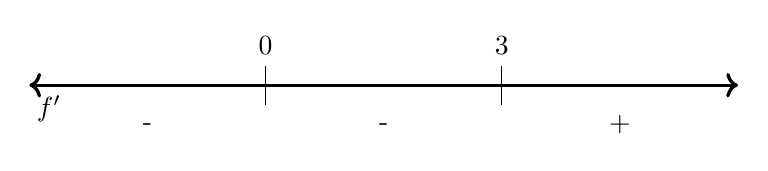
\begin{tikzpicture}
                    \draw[<->, very thick] (-4.5,0) -- (4.5,0); %number line
                    \draw (-1.5,0.25) -- (-1.5,-0.25); %Vertical tick marks
                    \draw (1.5,0.25) -- (1.5,-0.25);
                    \node () at (-4.25,-0.3) {$f'$}; %Labels
                    \node () at (-1.5,0.5) {0};
                    \node () at (1.5,0.5) {3};
                    \node () at (-3,-0.5) {-}; %Sign markings
                    \node () at (0,-0.5) {-};
                    \node () at (3,-0.5) {+};
                \end{tikzpicture}
            \end{center}

            \nonindent Since the derivative changes sign only at $x=3$,\\

            \begin{center}
                \begin{tabular}{cc}
                    if $x<3$ & $f'(x)\leq 0$ and $f$ is decreasing \\
                    If $x>3$ & $f'(x)> 0$ and $f$ is increasing
                \end{tabular}
            \end{center}


        \subsection{Extrema, Concavity, and Inflection Points}
            The curve of $y=f(x)$ has a \textbf{local/relative maximum} at a point where $x=c$ if
            $f(c)\geq f(x)$ for all $x$ in the immediate neighborhood of $c$. If a curve has a
            relative maximum at $x=c$, then the curve changes from increasing to decreasing as $x$
            increases through $c$. \\

            \noindent The curve of $y=f(x)$ has a \textbf{local/relative minimum} at a point where
            $x=c$ if $f(c)\leq f(x)$ for all $x$ in the immediate neighborhood of $c$.
            If a curve has a relative minimum at $x=c$, then the curve changes from decreasing to
            increasing as $x$ increases through $c$. \\

            \noindent If a function is differentiable on $[a,b]$ and has a relative extremum at $
            x=c, a<c<b$, then $f'(c)=0$. \\

            \noindent The \textbf{global/absolute maximum} of a function on $[a,b]$ occurs at $x=c$
            if $f(c)\geq f(x)$ for all $x$ on $[a,b]$. The \textbf{global/absolute minimum} of a
            function on $[a,b]$ occurs at $x=c$ if $f(c)\leq f(x)$ for all $x$ on $[a,b]$. \\

            \noindent A curve is \textbf{concave upward} on an interval $(a,b)$ if the curve lies
            above the tangent lines at each point in the interval $(a,b)$. A curve is
            \textbf{concave downward} on an interval $(a,b)$ if the curve lies below the tangent
            lines at each point in the interval $(a,b)$. \\

%    @TODO: Last tikzpicture won't load need to fix
            \begin{center}
                \begin{tabular}{|c|c|}
                    \hline
                    $f"(x) > 0$ & Concave Up \\
                    \hline
                    $f"(x) < 0$ & Concave Down \\
                    \hline
                \end{tabular}

                \begin{tabular}{cc}
                    \begin{tikzpicture} [scale = 0.75]
                        \begin{axis}[
                            axis lines = center,
                            xmin = -7,
                            xmax = 15,
                            ymin = 0,
                            ymax = 20
                        ]
                        \addplot[
                            color = red,
                            samples = 100,
                            domain = -7:15
                        ]
                        {((x-4)^2)/(4)+2};
                        \addplot[
                            dashed,
                            color = blue,
                            domain = -1.8:1.8,
                            samples = 2
                        ]
                        {-2*x+6};
                        \addplot[
                            dashed,
                            color = blue,
                            domain = 2.2:5.8,
                            samples = 2
                        ]
                        {2};
                        \addplot[
                            dashed,
                            color = blue,
                            domain = 6.2:9.8,
                            samples = 2
                        ]
                        {2*x-10};
                        \end{axis}
                    \end{tikzpicture}
                    &
                    \begin{tikzpicture} [scale=0.75]
                        \begin{axis}[
                            axis lines = center,
                            xmin = -7,
                            xmax = 15,
                            ymin = 0,
                            ymax = 20
                        ]
                        \addplot[
                            color = red,
                            samples = 100,
                            domain = -7:15
                        ]
                        {((x-4)^2)/(-4)+18};
                        \addplot[
                            dashed,
                            color = blue,
                            domain = -3.8:-0.2,
                            samples = 2
                        ]
                        {3*x+15};
                        \addplot[
                            dashed,
                            color = blue,
                            domain = 2.2:5.8,
                            samples = 2
                        ]
                        {18};
                        \addplot[
                            dashed,
                            color = blue,
                            domain = 8.2:11.8,
                            samples = 2
                        ]
                        {-3*x+39};
                        \end{axis}
                    \end{tikzpicture}
                \end{tabular}
            \end{center}


            \subsection{Optimization}
            \subsection{Graphically Relating a Function and its Derivatives}
            \subsection{Motion Along a Curve}
            \subsection{Tangent-Line Approximations}
            \subsection{The Newton-Raphson Method}
            \subsection{Related Rates}


    \pagebreak
%%%-------------------------------------------NEW SECTION--------------------------------------%%%

    \section{Integration}

        \subsection{Differentials}

    \section{Applications of Integration}
    \section{Introduction to Differential Equations}
    \section{Infinite Sequences and Series}

\end{document}